\documentclass[11pt,a4paper]{article}
\usepackage[utf8]{inputenc}
\usepackage[T1]{fontenc}
\usepackage{lmodern}
\usepackage[margin=2.2cm]{geometry}
\usepackage{amsmath}
\usepackage{booktabs}
\usepackage{tabularx}
\usepackage{graphicx}
\usepackage{enumitem}
\usepackage[hidelinks]{hyperref}
\usepackage{titlesec}

\graphicspath{{figs/}}
\setlist{itemsep=1pt,topsep=3pt}
\titlespacing*{\section}{0pt}{10pt}{4pt}
\setlength{\parskip}{4pt}
\setlength{\parindent}{0pt}
\newcommand{\var}[1]{\texttt{#1}}
\newcommand{\qs}{\var{quote\_signal}}
\newcommand{\mi}{\var{market\_index}}
\newcolumntype{L}{>{\raggedright\arraybackslash}X}

\begin{document}

{\Large\bfseries Freight Rate Prediction: Approach and Validation}\par
\vspace{2pt}
{\small Machine Learning Engineer assessment\\Code: \url{https://github.com/JanusAdamus/freight-rate-prediction}}\par
\vspace{6pt}

The final model predicts each load's rate with a mean absolute error of \textbf{\$42 (1.8\%)} on months it never saw, against \$88 for a lane-median baseline.  The decisions that matter most were about the data: two of the provided signals look predictive but fail on November--December, so the model leaves them out.

\section{Data split and validation approach}

The task is to predict November--December from January--October, so \textbf{all validation is split by time, never at random}.  A random split lets the model learn from days on both sides of each test day and overstates accuracy.  Each holdout answers one question:

\begin{table}[h]
\centering\small
\begin{tabularx}{\textwidth}{>{\raggedright\arraybackslash}p{2.7cm} >{\raggedright\arraybackslash}p{2.9cm} >{\raggedright\arraybackslash}p{3.4cm} L}
\toprule
Holdout & Train on & Evaluate on & Question it answers \\
\midrule
Time & Jan--Aug & Sep--Oct (9,523 loads) & Does it work on future months? \\
Time + unseen cities & Jan--Aug minus 8 random cities & Sep--Oct loads touching them; 20 draws & Does it work for new cities?  8 validation cities (12\% of loads) are absent from training. \\
August & Jan--Jul & August & Does it work when \qs\ is noise, as in Nov--Dec? \\
Rolling origin & months $< k$ & months $k$, $k{+}1$ & Do model choices hold across cut-offs? \\
\bottomrule
\end{tabularx}
\end{table}

\textbf{Statistical checks.}  Model comparisons use a Diebold--Mariano test on daily mean absolute errors with Newey--West variance (days, not loads, are the unit of dependence), backed by a Wilcoxon signed-rank test and Holm correction across the primary tests.  An adversarial classifier (Sep--Oct vs validation) reaches AUC 0.51 without coordinates, so apart from the new cities the validation loads look like recent training data.

\section{Key findings from the data}

\textbf{1. \qs\ switches meaning by month.}  It equals the true rate per mile ($\pm$1\%) in Jan, Feb, Mar, Jun and Sep, is inversely related to it in Apr, May, Jul and Oct, and is unrelated in August.  A per-day correlation between \qs\ and a quote-free model's prediction needs no labels, so it also classifies validation: November and December are noise months.  Their \qs\ distribution matches August's (Kolmogorov--Smirnov $p = 0.92$).

\begin{center}
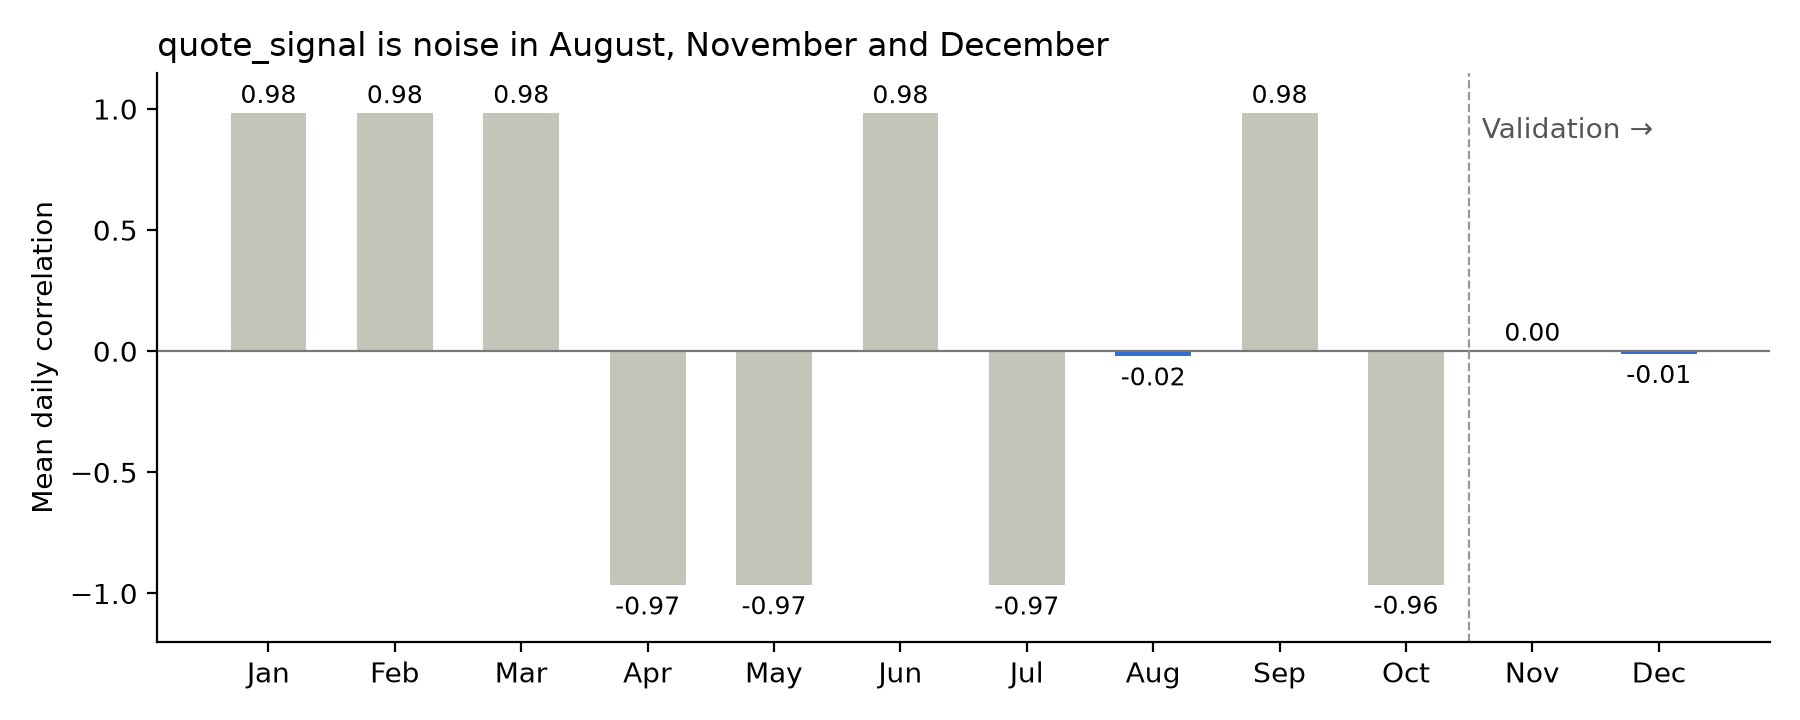
\includegraphics[width=0.8\textwidth]{quote_signal_regimes.png}
\end{center}

Including \qs\ looks excellent on Sep--Oct (\$32), only because September is a ``direct'' month.  On August it triples the error (\$114 vs \$40).  \textbf{It is excluded.}

\textbf{2. \mi\ does not generalise across months.}  It tracks daily prices within a month, but January and September share the same index (0.93 and 0.89) at different price levels (\$2.03 and \$2.16 per mile).  Adding it raises Sep--Oct MAE from \$42 to \$117.  Weekly-only, lagged, trend-adjusted and monotone versions did not help either.  \textbf{It is excluded.}

\textbf{3. Seasonality is real but not forecastable here.}  Prices vary 7.7\% across months (Kruskal--Wallis $p < 10^{-40}$) and 1.7\% by day of week.  No holiday effect was detected ($p = 0.09$).  No available input anticipates the Nov--Dec level, so the model predicts the yearly average level plus a day-of-week effect.

\section{Data-quality issues and how they were handled}

\begin{table}[h]
\centering\small
\begin{tabularx}{\textwidth}{L L L}
\toprule
Issue & Evidence & Handling \\
\midrule
1.4\% of rates are entry errors & Rate per mile at 0.2--0.4$\times$ or 2.4--4.7$\times$ the lane norm, with an empty gap in between.  In direct months, \qs\ for those loads is normal (0.99$\times$ the lane). & Dropped from training (outside \$1.2--\$4.0 per mile).  Metrics reported with and without them. \\
Negative weights (0.6\% train, 1.2\% validation) & In a regression of the price residual, the sign has no effect ($p = 0.84$) while $\log|\text{weight}|$ does. & Absolute value. \\
Missing weight and \mi & 300 and 374 rows in training. & Left as missing for the model. \\
Perturbed coordinates & Boston at latitude 39.3; longitudes clipped at $-69.5$, a latitude at 25.5. & Used as approximate positions, no city names. \\
Distance noise & Same lane has several distances; some rows at a 70-mile floor. & Kept; the model sees distance and detour ratio. \\
\bottomrule
\end{tabularx}
\end{table}

\section{Model}

\begin{itemize}
\item \textbf{Target:} $\log(\text{rate}/\text{distance})$.  It removes the distance scale and makes errors relative.  Prediction $= e^{\hat y}\times$ distance.
\item \textbf{Algorithm:} scikit-learn \var{HistGradientBoostingRegressor}, squared loss, 31 leaves, monotone constraints (heavier $\Rightarrow$ not cheaper; longer $\Rightarrow$ not pricier per mile).  Gradient boosting fits the non-linear distance curve and the lane $\times$ equipment $\times$ weight interactions.
\item \textbf{Features:} distance, pickup and delivery coordinates and their differences, straight-line distance, detour ratio, equipment, weight and day of week.  City names are left out so that unseen cities are priced from their location.
\item \textbf{Alternatives tested:} a ridge model with lane fixed effects, a two-stage ridge plus boosting, and boosting with lane target encoding.  All lost on unseen cities (MAE \$49--\$71).
\end{itemize}

\section{Results}

\begin{table}[h]
\centering\small
\begin{tabular}{lcccc}
\toprule
& \multicolumn{2}{c}{Time (Sep--Oct)} & Unseen cities & August \\
\cmidrule(lr){2-3}
Method & MAE & MAPE & MAE (20 draws) & MAE \\
\midrule
Lane-median baseline & \$88.15 & 3.74\% & \$185.20 & \$92.03 \\
\textbf{Final model} & \textbf{\$42.24} & \textbf{1.81\%} & \textbf{\$46.37} & \textbf{\$39.90} \\
Final + \mi & \$116.99 & 4.87\% & -- & \$66.44 \\
Final + \qs & \$32.00 & 1.31\% & -- & \$114.31 \\
\bottomrule
\end{tabular}
\end{table}

MAE and MAPE on rows with clean labels.  On all rows, including label errors, the final model's Sep--Oct MAE is \$98.  The model beats the baseline on every day of both time holdouts and in 20 of 20 unseen-city draws (sign test $p \approx 10^{-6}$).  Five random seeds move individual predictions by 0.28\% (median).  A split-conformal 80\% interval is $\pm$3.1\% and covered 82.7\% of October loads.

\section{December prediction chart}

\begin{center}
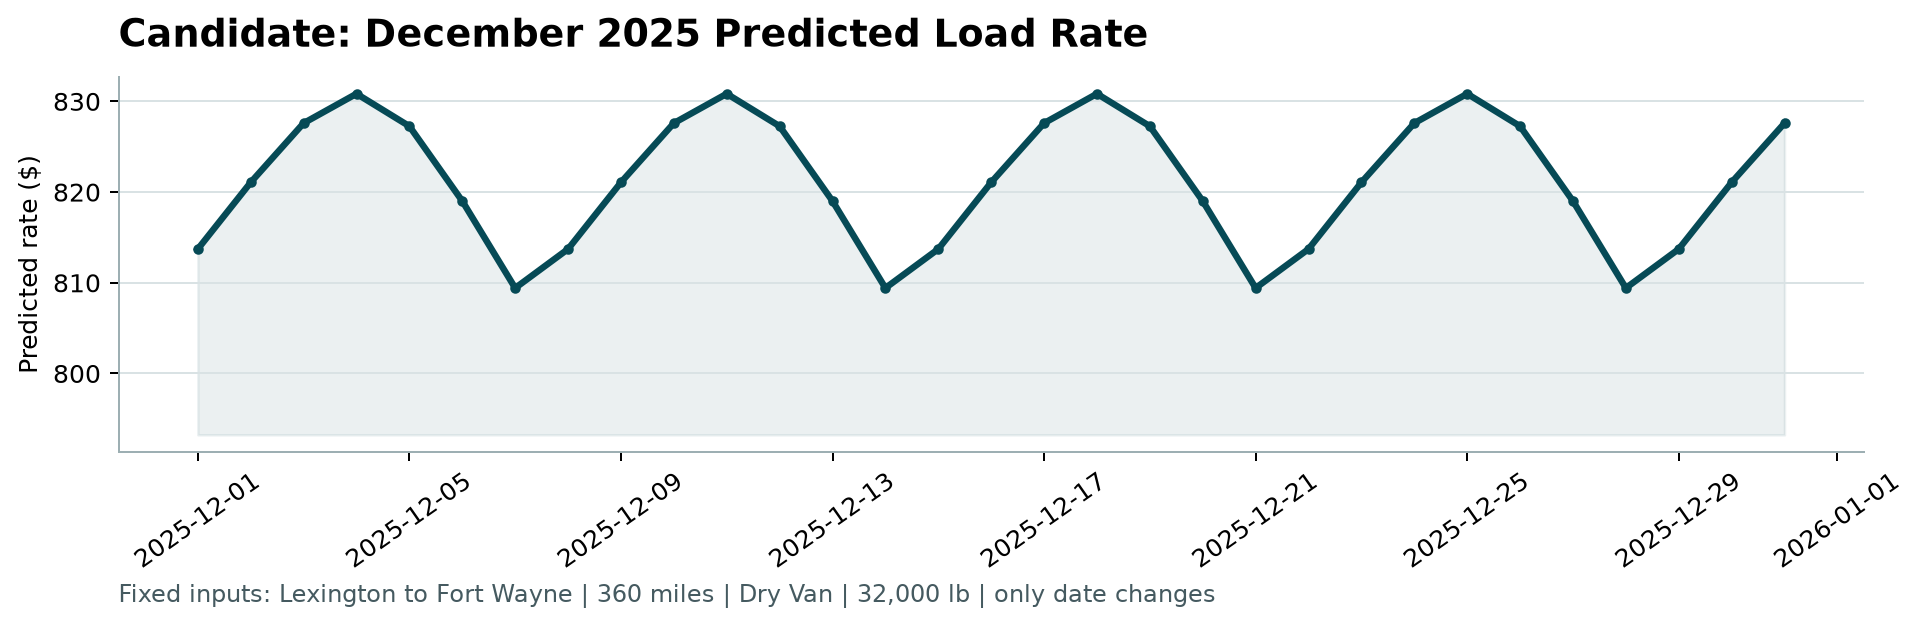
\includegraphics[width=0.95\textwidth]{candidate_december.png}
\end{center}

With lane, equipment, distance and weight fixed, only the date changes.  The model predicts \$809--\$831, highest on Thursdays and lowest on Sundays, matching the day-of-week pattern in the data.  The level matches the historical average for this lane in Dry Van (\$814).  The y-axis is zoomed in: the weekly swing is about $\pm$1.3\%.

\section{Limitations}

\begin{itemize}
\item \textbf{Nov--Dec level.}  If prices in those months run 2--3\% above or below the yearly average, all predictions shift together.  No November or December is in the training data, and none of the given signals anticipates it.
\item \textbf{Label errors in validation.}  If validation labels contain the same 1.4\% of entry errors, they will dominate squared-error metrics; the model targets the typical (median-like) rate.
\end{itemize}

\end{document}
